\chapter{Writing RISC-V Programs}

\ednote{Introduce the ISA register names and aliases in here?}%
This chapter introduces each of the RV32I instructions by developing programs
that demonstrate their usefulness.

\section{Use \texttt{ebreak} to Stop \rvddt{} Execution}
\index{Instruction!ebreak}
\label{uguide:ebreak}

It is a good idea to learn how to stop before learning how to go!

The \insn{ebreak} instruction exists for the sole purpose of transferring control back
to a debugging environment.\cite[p.~24]{rvismv1v22:2017}

When \rvddt{} executes an \insn{ebreak} instruction, it will immediately terminate any
executing {\em trace} or {\em go} command currently executing and return to the
command prompt without advancing the \reg{pc} register.

The machine language encoding shows that \insn{ebreak} has no operands.

\begin{figure}[H]
    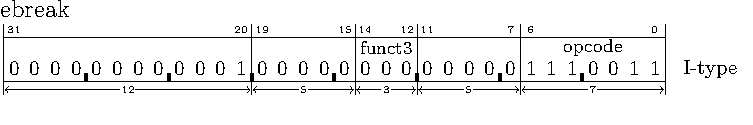
\includegraphics{figures/chapter04/ITypeEbreak.pdf}
\end{figure}

\listRef{examples/chapter04/ebreak/ebreak.out} demonstrates that since \rvddt{} does
not advance the \reg{pc} when it encounters an \insn{ebreak} instruction,
subsequent {\em trace} and/or {\em go} commands will re-execute the same \insn{ebreak}
and halt the simulation again (and again).
This feature is intended to help prevent overzealous users from accidently
running past the end of a code fragment.\footnote{This was one of the first {\em enhancements}
I needed for myself \tt:-)}

\listing{examples/chapter04/ebreak/ebreak.S}{A one-line \insn{ebreak} program.}

\listing{examples/chapter04/ebreak/ebreak.out}{\insn{ebreak} stopps \rvddt{} without advancing \reg{pc}.}


\section{Using the \insn{addi} Instruction}
\index{Instruction!addi}
\label{uguide:addi}

\ednote{Define what constant and immediate values are somewhere.}%
The detailed description of how the \insn{addi} instruction is executed
is that it:

\begin{enumerate}
    \item Sign-extends the immediate operand.
    \item Add the sign-extended immediate operand to the contents of the \reg{rs1} register.
    \item Store the sum in the \reg{rd} register.
    \item Add four to the \reg{pc} register (point to the next instruction.)
\end{enumerate}

In the following example \reg{rs1} = \reg{x28}, \reg{rd} = \reg{x29} and
the immediate operand is -1.

\begin{figure}[H]
    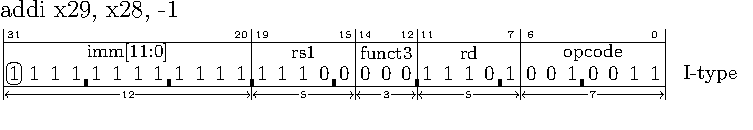
\includegraphics{figures/chapter04/IType-addi_x29_x28_-1.pdf}
\end{figure}

Depending on the values of the fields in this instruction a number of
different operations can be performed.  The most obvious is that it
can add things.  But it can also be used to copy registers, set a
register to zero and even, when you need to, accomplish nothing.

\subsection{No Operation}
\index{Instruction!nop}

It might seem odd but it is sometimes important to be able to execute
an instruction that accomplishes nothing while simply advancing the
\reg{pc} to the next instruction.  One reason for this is to fill
unused memory between two instructions in a program.%
\footnote{This can happen during the evolution of one portion of code
that reduces in size but has to continue to fit into a system without
altering any other code\ldots\ or sometimes you just need to waste
a small amount of time in a device driver.}

An instruction that accomplishes nothing is called a \insn{nop}
(sometimes systems call these \insn{noop}).  The name means
{\em no operation}.
The intent of a \insn{nop} is to execute without having any side effects
other than to advance the \reg{pc} register.

The \insn{addi} instruction can serve as a \insn{nop} by coding it like this:

\begin{figure}[H]
    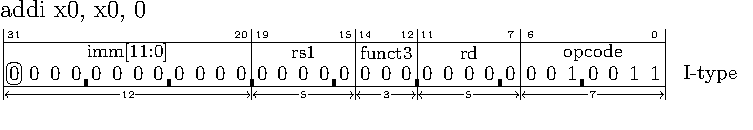
\includegraphics{figures/chapter04/IType-addi_x0_x0_0.pdf}
\end{figure}

The result will be to add zero to zero and discard the result (because you
can never store a value into the x0 register.)

The RISC-V assembler provides a pseudoinstruction specifically for this
purpose that you can use to improve the readability of your code.  Note
that the \insn{addi} and \insn{nop} instructions in \listRef{examples/chapter04/nop/nop.S}
are assembled into the exact same binary machine instructions
as can be seen by comparing it to
\verb@objdump@ \listRef{examples/chapter04/nop/nop.lst},
and \verb@rvddt@ \listRef{examples/chapter04/nop/nop.out} output.

%(The \hex{00000013} you can see are stored at addresses \hex{0} and \hex{4})
%as seen by looking at the \verb@objdump@ listing in \listRef{examples/chapter04/nop/nop.lst}.
%In fact, you can see that objdump shows both instructions as a \insn{nop}
%while \listRef{examples/chapter04/nop/nop.out} shows that \rvddt{} displays both as
%\verb@addi x0, x0, 0@.

\listing{examples/chapter04/nop/nop.S}{Demonstrate that \insn{addi} can be used as a \insn{nop}.}

\index{objdump}
\listing{examples/chapter04/nop/nop.lst}{Using \insn{addi} to perform a \insn{nop}}

\listing{examples/chapter04/nop/nop.out}{Using \insn{addi} to perform a \insn{nop}}


\subsection{Copying the Contents of One Register to Another}

By adding zero to one register and storing the sum in another register
the \insn{addi} instruction can be used to copy the value stored in one
register to another register.  The following instruction will copy
the contents of \reg{t4} into \reg{t3}.

\begin{figure}[H]
    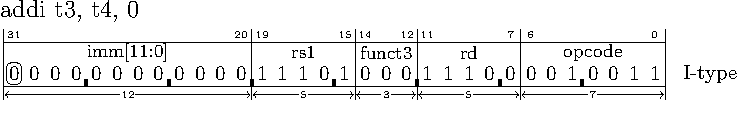
\includegraphics{figures/chapter04/IType-addi_t3_t4_0.pdf}
\end{figure}

\index{Instruction!mv}
This is a commonly required operation.  To make your intent clear
you may use the \insn{mv} pseudoinstruction for this purpose.

\listRef{examples/chapter04/mv/mv.S} shows the source of a program that is dumped in
\listRef{examples/chapter04/mv/mv.lst} illustrating that the assembler has generated the
same machine instruction (\hex{000e8e13} at addresses \hex{0} and \hex{4})
for both of the instructions.

\listing{examples/chapter04/mv/mv.S}{Comparing \insn{addi} to \insn{mv}}

\listing{examples/chapter04/mv/mv.lst}{An objdump of an \insn{addi} and \insn{mv} Instruction.}

\subsection{Setting a Register to Zero}

Recall that \reg{x0} always contains the value zero.  Any register
can be set to zero by copying the contents of \reg{x0} using \insn{mv}
(aka \insn{addi}).%
\footnote{There are other pseudoinstructions (such as \insn{li}) that can also
turn into an \insn{addi} instruction.  Objdump might display `{\tt addi t3,x0,0}'
as `{\tt mv t3,x0}' or `{\tt li t3,0}'.}

For example, to set \reg{t3} to zero:

\begin{figure}[H]
    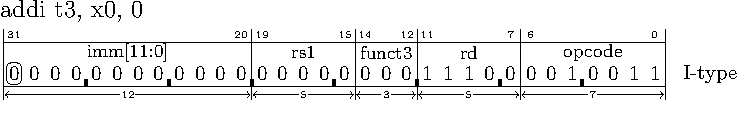
\includegraphics{figures/chapter04/IType_addi_t3_x0_0.pdf}
\end{figure}

\listing{examples/chapter04/mvzero/mv.S}{Using \insn{mv} (aka \insn{addi}) to zero-out a register.}

\listRef{examples/chapter04/mvzero/mv.out} traces the execution of the program in
\listRef{examples/chapter04/mvzero/mv.S} showing how \reg{t3} is changed from \hex{f0f0f0f0}
(seen on $\ell 16$) to \hex{00000000} (seen on $\ell 26$.)

\listing{examples/chapter04/mvzero/mv.out}{Setting \reg{t3} to zero.}


\subsection{Adding a 12-bit Signed Value}

\begin{figure}[H]
    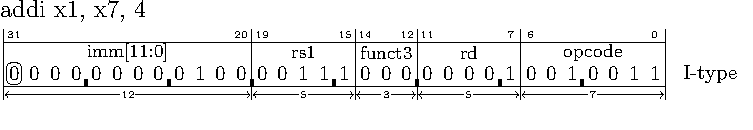
\includegraphics{figures/chapter04/IType_addi_x1_x7_4.pdf}
\end{figure}


{\small
\begin{verbatim}
    addi    t0, zero, 4     # t0 = 4
    addi    t0, t0, 100     # t0 = 104

    addi    t0, zero, 0x123     # t0 = 0x123
    addi    t0, t0, 0xfff       # t0 = 0x122 (subtract 1)

    addi    t0, zero, 0xfff     # t0 = 0xffffffff (-1)  (diagram out the chaining carry)
                                # refer back to the overflow/truncation discussion in binary chapter

	addi x0, x0, 0				# no operation (pseudo: nop)
	addi rd, rs, 0				# copy reg rs to rd (pseudo: mv rd, rs)
\end{verbatim}
}

\section{todo}

Ideas for the order of introducing instructions.


\section{Other Instructions With Immediate Operands}

\label{uguide:andi}
\label{uguide:ori}
\label{uguide:xori}
\label{uguide:slti}
\label{uguide:sltiu}
\label{uguide:srai}
\label{uguide:slli}
\label{uguide:srli}
{\small
\begin{verbatim}
    andi
    ori
    xori

    slti
    sltiu
    srai
    slli
    srli
\end{verbatim}
}

\section{Transferring Data Between Registers and Memory}

RV is a load-store architecture.  This means that the only way that the
CPU can interact with the memory is via the {\em load} and {\em store}
instructions.  All other data manipulation must be performed on register
values.

Copying values from memory to a register (first examples using regs set with addi):
\label{uguide:lb}
\label{uguide:lh}
\label{uguide:lw}
\label{uguide:lbu}
\label{uguide:lhu}
{\small
\begin{verbatim}
    lb
    lh
    lw
    lbu
    lhu
\end{verbatim}
}

Copying values from a register to memory:
\label{uguide:sb}
\label{uguide:sh}
\label{uguide:sw}
{\small
\begin{verbatim}
    sb
    sh
    sw
\end{verbatim}
}

\section{RR operations}
\label{uguide:add}
\label{uguide:sub}
\label{uguide:and}
\label{uguide:or}
\label{uguide:sra}
\label{uguide:srl}
\label{uguide:sll}
\label{uguide:xor}
\label{uguide:sltu}
\label{uguide:slt}
{\small
\begin{verbatim}
    add
    sub
    and
    or
    sra
    srl
    sll
    xor
    sltu
    slt
\end{verbatim}
}


\section{Setting registers to large values using lui with addi}

\label{uguide:lui}
\label{uguide:auipc}
{\small
\begin{verbatim}
    addi        // useful for values from -2048 to 2047
    lui         // useful for loading any multiple of 0x1000

    Setting a register to any other value must be done using a combo of insns:

    auipc       // Load an address relative the the current PC (see la pseudo)
    addi

    lui         // Load constant into into bits 31:12  (see li pseudo)
    addi        // add a constant to fill in bits 11:0
                    if bit 11 is set then need to +1 the lui value to compensate
\end{verbatim}
}


\section{Labels and Branching}

Start to introduce addressing here?

\label{uguide:beq}
\label{uguide:bne}
\label{uguide:blt}
\label{uguide:bge}
\label{uguide:bltu}
\label{uguide:bgeu}
\label{uguide:bgt}
\label{uguide:ble}
\label{uguide:bgtu}
\label{uguide:beqz}
\label{uguide:bnez}
\label{uguide:blez}
\label{uguide:bgez}
\label{uguide:bltz}
\label{uguide:bgtz}
{\small
\begin{verbatim}
    beq
    bne
    blt
    bge
    bltu
    bgeu

    bgt rs, rt, offset      # pseudo for: blt rt, rs, offset    (reverse the operands)
    ble rs, rt, offset      # pseudo for: bge rt, rs, offset    (reverse the operands)
    bgtu rs, rt, offset     # pseudo for: bltu rt, rs, offset   (reverse the operands)
    bleu rs, rt, offset     # pseudo for: bgeu rt, rs, offset   (reverse the operands)

    beqz rs, offset         # pseudo for: beq rs, x0, offset
    bnez rs, offset         # pseudo for: bne rs, x0, offset
    blez rs, offset         # pseudo for: bge x0, rs, offset
    bgez rs, offset         # pseudo for: bge rs, x0, offset
    bltz rs, offset         # pseudo for: blt rs, x0, offset
    bgtz rs, offset         # pseudo for: blt x0, rs, offset
\end{verbatim}
}



\section{Jumps}

Introduce and present subroutines but not nesting until introduce stack operations.

\label{uguide:jal}
\label{uguide:jalr}
{\small
\begin{verbatim}
    jal
    jalr
\end{verbatim}
}



\section{Pseudoinstructions}

{\small
\begin{verbatim}
    li   rd,constant
                     lui      rd,(constant + 0x00000800) >> 12
                     addi     rd,rd,(constant & 0x00000fff)

    la   rd,label
                     auipc    rd,((label-.) + 0x00000800) >> 12
                     addi     rd,rd,((label-(.-4)) & 0x00000fff)

    l{b|h|w} rd,label
                     auipc    rd,((label-.) + 0x00000800) >> 12
                     l{b|h|w} rd,((label-(.-4)) & 0x00000fff)(rd)

    s{b|h|w} rd,label,rt          # rt used as a temp reg for the operation (default=x6)
                     auipc    rt,((label-.) + 0x00000800) >> 12
                     s{b|h|w} rd,((label-(.-4)) & 0x00000fff)(rt)

    call label       auipc    x1,((label-.) + 0x00000800) >> 12
                     jalr     x1,((label-(.-4)) & 0x00000fff)(x1)

    tail label,rt                 # rt used as a temp reg for the operation (default=x6)
                     auipc    rt,((label-.) + 0x00000800) >> 12
                     jalr     x0,((label-(.-4)) & 0x00000fff)(rt)

    mv   rd,rs       addi     rd,rs,0

    j    label       jal      x0,label
    jal  label       jal      x1,label
    jr   rs          jalr     x0,0(rs)
    jalr rs          jalr     x1,0(rs)
    ret              jalr     x0,0(x1)
\end{verbatim}
}

\subsection{The \texttt{li} Pseudoinstruction}

Note that the \texttt{li} pseudoinstruction includes an (effectively) conditional addition
of 1 to the immediate operand
in the \texttt{lui} instruction.  This is because the immediate operand in the
\texttt{addi} instruction is sign-extended before it is added to \verb@rd@.
If the immediate operand to the \texttt{addi} has its most-significant-bit set to 1 then
it will have the effect of subtracting 1 from the operand in the \verb@lui@ instruction.

Consider the case of putting the value \texttt{0x12345800} into register \texttt{x5}:

{\small
\begin{verbatim}
    li  x5,0x12345800
\end{verbatim}
}
{\color{red}
A naive (incorrect) solution might be:
{\small
\begin{verbatim}
    lui  x5,0x12345    // x5 = 0x12345000
    addi x5,x5,0x800   // x5 = 0x12345000 + sx(0x800) = 0x12345000 + 0xfffff800 = 0x12344800
\end{verbatim}
}
The result of the above code is that an incorrect value has been placed into x5.
}

To remedy this problem, the value used in the \texttt{lui} instruction can be altered
(by adding 1 to its operand) to compensate for the sign-extention in the \texttt{addi}
instruction:
{\small
\begin{verbatim}
    lui  x5,0x12346    // x5 = 0x12346000  (note: this is 0x12345800 + 0x0800)
    addi x5,x5,0x800   // x5 = 0x12346000 + sx(0x800) = 0x12346000 + 0xfffff800 = 0x12345800
\end{verbatim}
}

Keep in mind that the \texttt{li} pseudoinstruction must {\em only} increment the operand
of the \texttt{lui} instruction when it is known that the operand of the subsequent
\texttt{addi} instruction will be a negative number.

\ednote{Add a ribbon diagram of this?}%
By adding \texttt{0x00000800} to the immediate operand of the \texttt{lui} instruction in
this example, a carry-bit into bit-12 will be set to \texttt{1} iff the value in
bits 11-0 will be treated as a negative value in the subsequent \texttt{addi} instruction.
In other words, when bit-11 is set to \texttt{1} in the immediate operand of the \texttt{li}
pseudoinstruction, the immediate operand of the \texttt{lui} instruction will be
incremented by \texttt{1}.

Consider the case where we wish to put the value \texttt{0x12345700} into register \texttt{x5}:
{\small
\begin{verbatim}
    lui  x5,0x12345    // x5 = 0x12345000  (note that 0x12345700 + 0x0800 = 0x12345f00)
    addi x5,x5,0x700   // x5 = 0x12345000 + sx(0x700) = 0x12345000 + 0x00000700 = 0x12345700
\end{verbatim}
}
The sign-extension in this example performed by the \texttt{addi} instruction will convert the
\texttt{0x700} to \texttt{0x00000700} before the addition.

Observe that \texttt{0x12345700+0x0800 = 0x12345f00} and therefore, after shifting
to the right, the least significant \texttt{0xf00} is truncated, leaving \texttt{0x12345} as
the immediate operand of the \texttt{lui} instruction.  The addition of
\texttt{0x0800} in this example has no effect on the immediate operand of the \texttt{lui}
instruction because bit-11 in the original value \texttt{0x12345700} is zero.

A general algorithm for implementing the \texttt{li rd,constant} pseudoinstruction is:

{\small
\begin{verbatim}
    lui  rd,(constant + 0x00000800) >> 12
    addi rd,rd,(constant & 0x00000fff)		// the 12-bit immediate is sign extended
\end{verbatim}
}

\ednote{Find a proper citation for this.}%
Note that on RV64 and RV128 systems, the \texttt{lui} places the immediate operand into
bits 31-12 and then sign-extends the result to \texttt{XLEN} bits.

\subsection{The \texttt{la} Pseudoinstruction}

The \verb@la@ (and others that use \verb@auipc@ such as
the \verb@l{b|h|w}@, \verb@s{b|h|w}@, \verb@call@, and \verb@tail@) pseudoinstructions
also compensate for a sign-ended negative number when adding a 12-bit immediate
operand. The only difference is that these use a \verb@pc@-relative addressing mode.

For example, consider the task of putting an address represented by the label \verb@var1@
into register x10:

{\small
\begin{verbatim}
00010040     la     x10,var1
00010048 ...                 # note that the la pseudoinstruction expands into 8 bytes
...

         var1:
00010900     .word  999       # a 32-bit integer constant stored in memory at address var1
\end{verbatim}
}
The \verb@la@ instruction in this example will expand into:
{\small
\begin{verbatim}
00010040     auipc x10,((var1-.) + 0x00000800) >> 12
00010044     addi  x10,x10,((var1-(.-4)) & 0x00000fff)
\end{verbatim}
}

Note that \verb@auipc@ will shift the immediate operand to the left 12 bits and then
add that to the \verb@pc@ register (see \autoref{insn:auipc}.)

The assembler will calculate the value of \verb@(var1-.)@ by subtracting the address
represented by the label \verb@var1@ from the address of the current instruction
(which is expressed as '.') resulting in the number of bytes from the current instruction
to the target label\ldots{} which is \verb@0x000008c0@.

Therefore the expanded pseudoinstruction example will become:
{\small
\begin{verbatim}
00010040     auipc x10,((0x00010900 - 0x00010040) + 0x00000800) >> 12
00010044     addi  x10,x10,((0x00010900 - (0x00010044 - 4)) & 0x00000fff)   # note the extra -4 here!
\end{verbatim}
}
After performing the subtractions, it will reduce to this:
{\small
\begin{verbatim}
00010040     auipc x10,(0x000008c0 + 0x00000800) >> 12
00010044     addi  x10,x10,(0x000008c0 & 0x00000fff)
\end{verbatim}
}
Continuing to reduce the math operations we get:
{\small
\begin{verbatim}
00010040     auipc x10,0x00001              # 0x000008c0 + 0x00000800 = 0x000010c0
00010044     addi  x10,x10,0x8c0
\end{verbatim}
}

Note that the \verb@la@ pseudoinstruction exhibits the same sort of technique as
the \verb@li@ in that
if/when the immediate operand of the \verb@addi@ instruction has its most significant
bit set then the operand in the \verb@auipc@ has to be incremented by 1 to compensate.








\section{Relocation}

Because expressions that refer to constants and address labels are common in
assembly language programs, a shorthand notation is available for calculating
the pairs of values that are used in the implementation of things like the
\verb@li@ and \verb@la@ pseudoinstructions (that have to be written to
compensate for the sign-extension that will take place in the immediate operand
that appears in instructions like \verb@addi@ and \verb@jalr@.)

\subsection{Absolute Addresses}

To refer to an absolute value, the following operators can be used:
{\small
\begin{verbatim}
    %hi(constant)    // becomes: (constant + 0x00000800) >> 12
    %lo(constant)    // becomes: (constant & 0x00000fff)
\end{verbatim}
}

Thus, the \verb@li@ pseudoinstruction can, therefore, be expressed like this:

{\small
\begin{verbatim}
    li   rd,constant  lui      rd,%hi(constant)
                      addi     rd,rd,%lo(constant)
\end{verbatim}
}



\subsection{PC-Relative Addresses}

The following can be used for PC-relative addresses:
{\small
\begin{verbatim}
    %pcrel_hi(symbol) // becomes: ((symbol-.) + 0x0800) >> 12
    %pcrel_lo(lab)    // becomes: ((symbol-lab) & 0x00000fff)
\end{verbatim}
}

Note the subtlety involved with the \verb@lab@ on \verb@%pcrel_lo@. It is needed to
determine the address of the instruction that contains the corresponding \verb@%pcrel_hi@.
(The label \verb@lab@ MUST be on a line that used a \verb@%pcrel_hi()@ or get an
error from the assembler.)

Thus, the \verb@la rd,label@ pseudoinstruction can be expressed like this:
{\small
\begin{verbatim}
xxx:  auipc rd,%pcrel_hi(label)
      addi  rd,rd,%pcrel_lo(xxx)  // the xxx tells pcrel_lo where to find the matching pcrel_hi
\end{verbatim}
}

Examples of using the \verb@auipc@ \& \verb@addi@ together with \verb@%pcrel_hi()@ and
\verb@%pcrel_lo()@:

{\small
\begin{verbatim}
xxx:    auipc   t1,%pcrel_hi(yyy)     // ((yyy-.) + 0x0800) >> 12
        addi    t1,t1,%pcrel_lo(xxx)  // ((yyy-xxx) & 0x00000fff)
...
yyy:                                  // the address: yyy is saved into t1 above
...
\end{verbatim}
}


Referencing the same \verb@%pcrel_hi@ in multiple subsequent uses of \verb@%pcrel_lo@ is legal:
{\small
\begin{verbatim}
label:  auipc   t1,%pcrel_hi(symbol)
        addi    t2,t1,%pcrel_lo(label)   // t2 = symbol
        addi    t3,t1,%pcrel_lo(label)   // t3 = symbol
        lw      t4,%pcrel_lo(label)(t1)  // t4 = fetch value from memory at 'symbol'
        addi    t4,t4,123                // t4 = t4 + 123
        sw      t4,%pcrel_lo(label)(t1)  // store t4 back into memory at 'symbol'
\end{verbatim}
}

\section{Relaxation}

%\ednote{I'm not sure I want to get into the details of how this is done. Just assume it works.}%
In the simplest of terms, {\em Relaxation} refers to the ability of the
linker (not the compiler!) to determine if/when the instructions that
were generated with the \verb@xxx_hi@ and \verb@xxx_lo@ operators are
unneeded (and thus waste execution time and memory) and can therefore
be removed.

However, doing so is not trivial as it will result in moving things around
in memory, possibly changing the values of address labels in the
already-assembled program!  Therefore, while the motivation for
rexation is obvious, the process of implementing it is non-trivial.

See: \url{https://github.com/riscv/riscv-elf-psabi-doc/blob/master/riscv-elf.md}